\documentclass[11pt]{beamer}

% Packages
\usepackage{graphicx}
\usepackage{hyperref}
\usepackage{listings}
\usepackage{color}
\usepackage{tikz}
\usepackage{amsmath}
\usepackage{amssymb}
\usepackage{helvet} 
\usepackage{caption}
\usepackage{bookmark}

\usetikzlibrary{positioning}

% Beamer settings
\usetheme{metropolis}
\usecolortheme{default}

% Document settings
\title{TFE25-462: Meeting 3}
\subtitle{Programming USRP X310 with UHD and RFNoC}
\author{Quentin Prieels}
\date{\today}


\begin{document}

% Title slide
\maketitle

% Table of contents
\begin{frame}
    \frametitle{Table of contents}
    \tableofcontents
\end{frame}

%%%%%%%%%%%%%%%%%%%%%%%%%%
% PART 1: Setup overview %
%%%%%%%%%%%%%%%%%%%%%%%%%%
\section{Setup overview}

% Slide 1: Setup overview block diagram
\begin{frame}
    \frametitle{Setup overview}
    \begin{figure}
        %\centering
        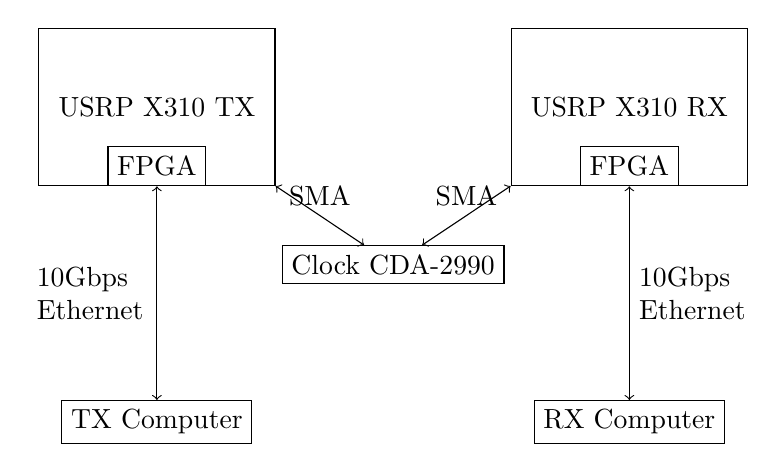
\begin{tikzpicture}
            %% Devices
            % TX and RX computers
            \node[draw, rectangle] (tx) at (-3, -2) {TX Computer}; 
            \node[draw, rectangle] (rx) at (3, -2) {RX Computer};
           

            % USRP X310 TX and RX - with FPGA inside (rectangle inside de USRP rectangle)
            \node[draw, rectangle, minimum width=3cm, minimum height=2cm] (tx_usrp) at (-3, 2) {USRP X310 TX};
            \node[draw, rectangle, minimum width=1cm, minimum height=0.5cm, anchor=south] at (tx_usrp.south) {FPGA};
            
            \node[draw, rectangle, minimum width=3cm, minimum height=2cm] (rx_usrp) at (3, 2) {USRP X310 RX};
            \node[draw, rectangle, minimum width=1cm, minimum height=0.5cm, anchor=south] at (rx_usrp.south) {FPGA};
        
            %\node[draw, rectangle] (tx_fpga) at (4, -2.5) {FPGA};

            % Clock to connect the USRP X310
            \node[draw, rectangle] (clock) at (0, 0) {Clock CDA-2990};

            %% Connections
            % RX and TX computers to USRP X310 (10Gbps Ethernet)
            \draw[<->] (tx) -- (tx_usrp) node[midway, left] {\parbox{1.4cm}{10Gbps\\Ethernet}};
            \draw[<->] (rx) -- (rx_usrp) node[midway, right] {\parbox{1cm}{10Gbps\\Ethernet}};
            
            % USRP X310 to Clock (SMA)
            \draw[<->] (tx_usrp) -- (clock) node[midway, above] {SMA};
            \draw[<->] (rx_usrp) -- (clock) node[midway, above] {SMA};

        \end{tikzpicture}
        \caption{Setup block diagram}
    \end{figure}
\end{frame}

%%%%%%%%%%%%%%%%%%%%%%%%%%%%%%%%%%%%%%%%%%%%%%%%%%%%
% PART 2: USRP Components and programming overview %
%%%%%%%%%%%%%%%%%%%%%%%%%%%%%%%%%%%%%%%%%%%%%%%%%%%%
\section{USRP Components and programming overview}

% Slide 2: USRP Components and programming overview
\begin{frame}
    \frametitle{USRP Overview}
    \begin{itemize}
        \item Two denominations: 
        \begin{itemize}
            \item \textbf{USRP X310} in the Ettus Research product line.
            \item \textbf{USRP 2944R} in the National Instruments product line.
        \end{itemize}
        \item It includes on the Xilinx Kintex-7 FPGA.
        \item It can be programmed using the UHD driver and RFNoC provided by Ettus Research (see later)
        \item Needs AMD Xilinx Vivado to compile the FPGA image.
    \end{itemize}
\end{frame}

% Slide 3: USRP Block Diagram
\begin{frame}
    \frametitle{USRP Block Diagram}
    \begin{figure}
        \centering
        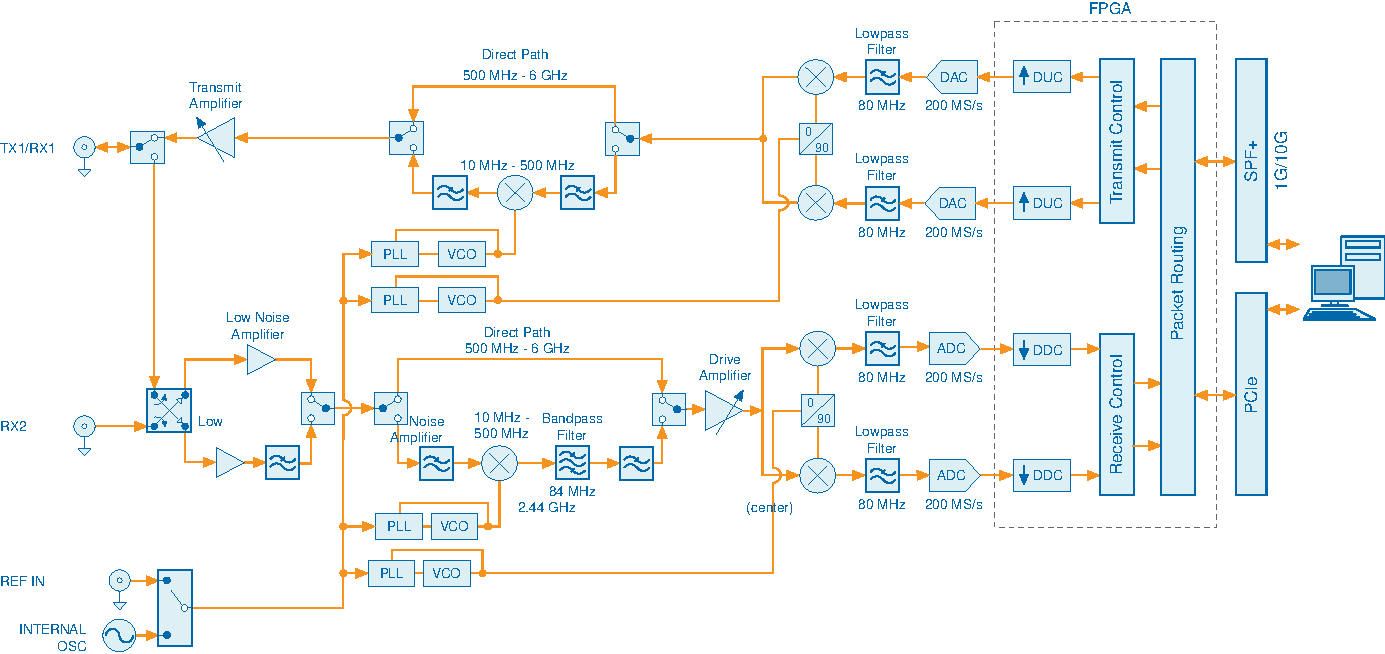
\includegraphics[width=\textwidth]{usrp_block_diagram.pdf}
        \caption{USRP X310 Block Diagram}
    \end{figure}
\end{frame}

% Slide 4: UHD Overview
\begin{frame}
    \frametitle{UHD Overview}
    \begin{itemize}
        \item UHD stands for \textbf{USRP Hardware Driver}.
        \item It is an open-source, cross-platform driver for USRP devices.
        \item It is written in C++ and provides a C API.
        \item It is used to control the USRP device and stream data to and from it.
        \item It is used to program and manage the FPGA image.
    \end{itemize}
\end{frame}

% Slide 5: RFNoC Overview
\begin{frame}
    \frametitle{RFNoC Overview}
    \begin{itemize}
        \item RFNoC stands for \textbf{RF Network on Chip}.
        \item It is a framework that allows to create FPGA blocks that can be connected together.
        \item It comes with a set of blocks that are already implemented and can be used.
        \item It is includes in the UHD driver since version 3.15, and cannot be disabled since version 4.0.
    \end{itemize}
\end{frame}

% Slide 6: RFNoC Block Diagram
\begin{frame}
    \frametitle{RFNoC Block Diagram}
    \begin{figure}
        \centering
        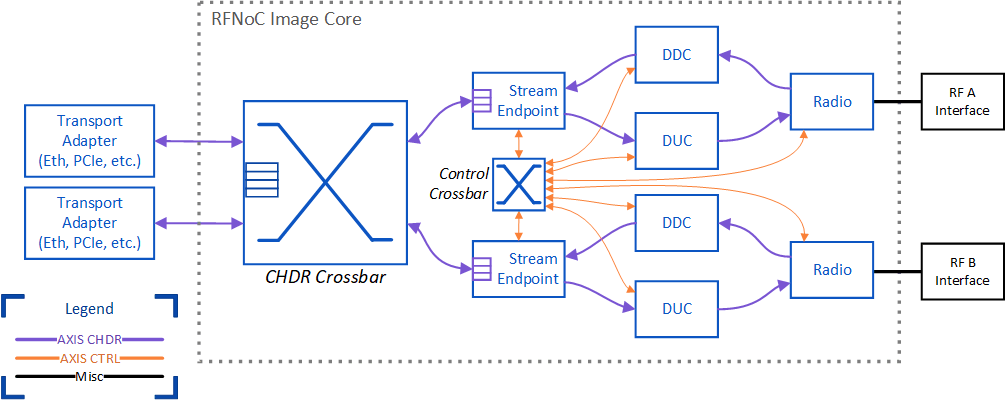
\includegraphics[width=\textwidth]{simplified_rfnoc_image_uhd_4.png}
        \caption{RFNoC Block Diagram}
    \end{figure}
\end{frame}


%%%%%%%%%%%%%%%%%%%%%%%%%%%%%%%%%%%%%%%%%%%%%%%%%%%%
% PART 2: Toolchain and programming environment    %
%%%%%%%%%%%%%%%%%%%%%%%%%%%%%%%%%%%%%%%%%%%%%%%%%%%%

\section{Tool chain and programming environment}

% Slide 7: Toolchain proposed by Ettus Research
\begin{frame}
    \frametitle{Tool chain proposed by Ettus Research}
    \begin{itemize}
        \item Ettus suggest the following tool chain to program the USRP X310:
        \item It includes:
        \begin{itemize}
            \item \textbf{UHD}: to control the USRP device and stream data.
            \item \textbf{RFNoC}: to create FPGA blocks and connect them.
            \item \textbf{Xilinx Vivado} 2021.1 with AR76780 patch: to compile the FPGA image.
            \item Optional \textbf{GNU Radio}: to create the signal processing flow.
        \end{itemize}
        \item Ubuntu 20.04 recommended, with a lot of dependencies.
        \item All on the same computer.
    \end{itemize}
\end{frame}

% Slide 8: Toolchain in practice
\begin{frame}
    \frametitle{Toolchain in practice}
    \begin{itemize}
        \item What we have now:
        \begin{itemize}
            \item \textbf{UHD 4.1.0.5} installed on RX computers.
            \item \textbf{Vivado 2022.1} installed on workstation.
        \end{itemize}
        \item What we need to do:
        \begin{itemize}
            \item Install UHD on workstation to be able to compile the FPGA image (and all its dependencies)
            \item Update UHD on RX computers to the latest version (have common version on all computers).
            \item Check if the AR76780 patch is needed for Vivado 2022.1.
        \end{itemize}
    \end{itemize}
\end{frame}

%%%%%%%%%%%%%%%%%%%%%%%%%%%%%%%%%%%%%%%%%%%%%%%%%%%%
% PART 3: ToDOs                                   %
%%%%%%%%%%%%%%%%%%%%%%%%%%%%%%%%%%%%%%%%%%%%%%%%%%%%

\section{Next steps}

% Slide 9: ToDOs
\begin{frame}
    \frametitle{Next steps}
    \begin{enumerate}
        \item Install / Update software on all computers.
        \item Update the FPGA image on the USRP X310 with the latest one.
        \item Check toolchain
        \item Continue with RFNoC tutorials to compile and run the examples.
        \item Start developing the custom blocks needed for this TFE.
    \end{enumerate}
\end{frame}

% Slide 10: Poster session INFO
\begin{frame}
    \frametitle{INFO poster session}
    \begin{itemize}
        \item The poster session will take place on \textbf{December 4}.
        \item Deadline on \textbf{November 27} to send the poster.
        \item Purpose:
        \begin{itemize}
            \item  Present the work achieved so far.
            \item Present topic and plan for this year.
        \end{itemize}
    \end{itemize}
\end{frame}

\end{document}
